\documentclass[a4paper,14pt]{extarticle} \usepackage[utf8]{inputenc}
\usepackage[T1]{fontenc}
\usepackage[margin=2.5cm]{geometry}

% Fonte Caladea se existir, senão lmodern
\IfFileExists{caladea.sty}{
  \usepackage{caladea}
}{
  \usepackage{lmodern} }
\usepackage{ragged2e}
\usepackage{graphicx}
\usepackage[portuguese]{babel}
\usepackage{wrapfig}
\usepackage{hyperref}
\usepackage{fancyhdr}
\usepackage{xcolor}
\usepackage{rotating}
\usepackage{titlesec}
\usepackage{epigraph}
\usepackage{dirtytalk}
\usepackage{indentfirst} % Indenta o primeiro parágrafo após seções

% Ajuste do recuo de parágrafo
\setlength{\parindent}{1.5em}

% Adjust headheight to remove LaTeX warning
\setlength{\headheight}{17.54163pt}

% Centralizar títulos
\titleformat{\section}
  {\normalfont\centering\bfseries\Large}{}{1em}{}

\titleformat{\subsection}
  {\normalfont\centering\bfseries\large}{}{1em}{}

\titleformat{\subsubsection}
  {\normalfont\centering\bfseries}{}{1em}{}

% -------------- Símbolos de Versículo e Resposta --------------
% Definição do símbolo (a “barrinha” inclinada)
\makeatletter
\newcommand{\vers@resp@sym}{%
  \raisebox{0.2ex}{\rotatebox[origin=c]{-20}{$\m@th\rceil$}}%
}
% macro interna que sobrepõe a barrinha e a letra V ou R
\newcommand{\vers@resp}[2]{%
  {\ooalign{%
     \hidewidth\kern#1\vers@resp@sym\hidewidth\cr
     #2\cr
  }}%
}
% comandos públicos \versicle e \response
\DeclareRobustCommand{\versicle}{\vers@resp{-0.1em}{V}}
\DeclareRobustCommand{\response}{\vers@resp{0pt}{R}}
\makeatother
% ^------------- Símbolos de Versículo e Resposta -------------^

% Rodapé com imagem e página
\pagestyle{fancy}
% ---- Cabeçalho ------------
\fancyhf[C]{}
% ----- Rodapé --------------
\fancyfoot[C]{%
  
\includegraphics[scale=0.2]{assets/cross.png}\quad
  \textit{\textit{Santos Marcos Chong e Aleixo Se-yong, Rogai por Nós}}\quad
  \thepage
}

\usepackage{pdfpages}
\begin{document}
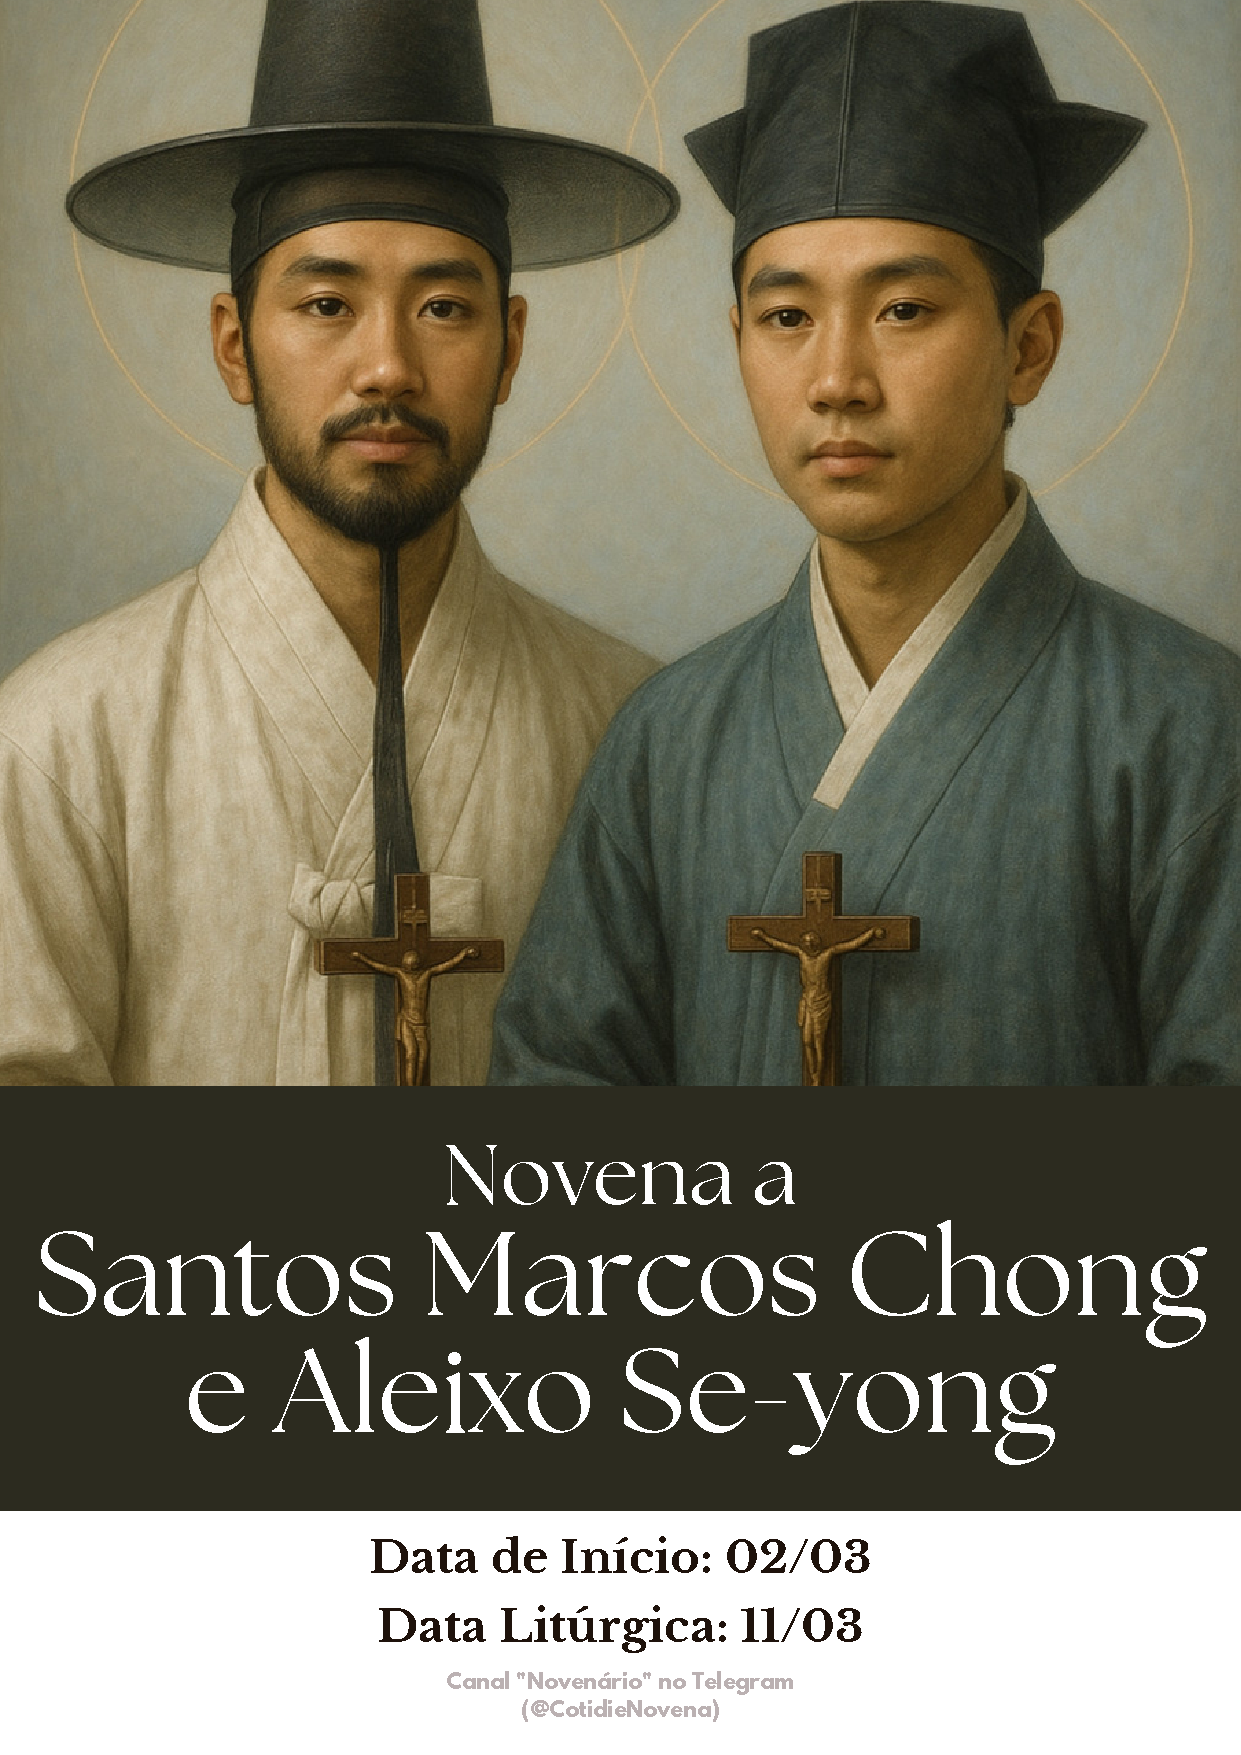
\includepdf[pages=1]{Capa Santos Marcos Chong e Aleixo Se-yong.pdf}

\begin{center}
  {\huge Novena de Santos Marcos Chong e Aleixo Se-yong}
\end{center}



\noindent\rule{\textwidth}{0.4pt}

\tableofcontents

\thispagestyle{empty}


% --- Origem ---
\newpage

\section{História}


\subsection{Origens e fé nascente na Coreia}

 No século XIX, a Coreia vivia um tempo de isolamento político e de forte perseguição à fé cristã. Foi nesse contexto que floresceu o testemunho de Marcos Chong Ui-bae e Aleixo Se-yong, dois fiéis leigos que, iluminados pela graça de Deus, abraçaram o Evangelho com fidelidade até o martírio. Ambos pertencem à geração de católicos coreanos que, mesmo sem presença contínua de missionários, mantiveram viva a Igreja através da oração, do estudo das Escrituras e da comunhão fraterna.

\subsection{Vida e vocação cristã de Marcos Chong Ui-bae}

 Marcos Chong nasceu em 1771, em uma família nobre da região de Chungcheong. Converteu-se ao cristianismo na juventude, após ouvir falar dos ensinamentos de Cristo trazidos por estudiosos leigos. Admirava a justiça, a humildade e a misericórdia ensinadas no Evangelho. Após o batismo, dedicou-se a instruir outros na fé, sendo reconhecido como homem prudente, de palavra calma e coração compassivo. Era casado e pai de família, e via na vida doméstica uma oportunidade de viver a caridade e o serviço.

 \subsection{Vida e testemunho de Aleixo Se-yong}

 Aleixo Se-yong nasceu alguns anos depois, em uma família também convertida ao cristianismo. Desde jovem revelou fervor extraordinário e desejo de servir. Quando as perseguições começaram a se intensificar, Aleixo dedicava-se a fortalecer os fiéis, animando-os a perseverar. Sabia dos riscos, mas dizia: "Antes morrer por Cristo do que viver sem Ele." Era homem simples, mas de fé firme e coração ardente.

 \subsection{Perseguição e prisão}

 Durante a grande perseguição de 1801, o governo coreano reprimiu violentamente a comunidade católica, acusando os cristãos de trair as tradições do país. Marcos e Aleixo foram presos por se recusarem a renegar a fé e por acolherem missionários estrangeiros. Submetidos a interrogatórios e torturas, permaneceram inabaláveis. As autoridades prometeram liberdade se renunciassem a Cristo; ambos responderam com serenidade que preferiam morrer fiéis a Ele.

 \subsection{O martírio pela fé}

 Depois de longos tormentos, foram condenados à morte. Marcos Chong foi executado primeiro, em 27 de agosto de 1801, aos trinta anos de idade. Morreu rezando e perdoando os algozes. Aleixo Se-yong, mais jovem, foi decapitado logo em seguida, proclamando o nome de Jesus. Os cristãos que testemunharam sua morte relataram que seus rostos, banhados de sangue, permaneciam serenos, como quem já contemplava o céu.

 \subsection{Testemunho e frutos espirituais}

 O sacrifício de Marcos e Aleixo não foi em vão. Seu sangue derramado tornou-se semente de fé na Coreia, fortalecendo os irmãos perseguidos e inspirando novas gerações de cristãos. Eles são lembrados como exemplos de leigos santos, que sem títulos ou cargos, mostraram com a vida que o amor a Cristo vale mais que a própria existência.

 \subsection{Reconhecimento e canonização}

 A Igreja reconheceu oficialmente a santidade de Marcos Chong Ui-bae e Aleixo Se-yong junto com outros mártires coreanos. Foram beatificados pelo Papa Pio XI em 1925 e canonizados por São João Paulo II em 6 de maio de 1984, em Seul, na cerimônia que glorificou 103 mártires da Coreia. Sua memória litúrgica é celebrada em 20 de setembro.

 \subsection{Virtudes e espiritualidade}

 Esses santos coreanos viveram a fé com pureza, humildade e coragem silenciosa. Uniram-se profundamente à cruz de Cristo e confiaram na misericórdia divina. Sua espiritualidade é marcada pela oração constante, pela fidelidade à verdade e pela disposição em perdoar os perseguidores. Ensinam que o martírio não é apenas um ato de morte, mas uma entrega de amor total.

 \subsection{Representação}

 Nas imagens sagradas, Marcos Chong e Aleixo Se-yong aparecem vestidos com as túnicas coreanas tradicionais, de cor branca, símbolo da pureza, e segurando o crucifixo - sinal da vitória de Cristo. São representados lado a lado, em atitude de oração e serenidade, recordando a fraternidade que os uniu até o fim.

 \subsection{Devoção e intercessão}

 A devoção aos mártires coreanos é viva em todo o Oriente e se espalha hoje por comunidades cristãs do mundo inteiro. Marcos e Aleixo são invocados como intercessores da coragem na fé, da fidelidade à Igreja e da esperança em tempos de provação. Inspiram os leigos a viver o Evangelho no cotidiano com alegria e perseverança.

% --- Orações Diárias ---
\newpage

\vfill

\section{Orações}
\subsection{Oração Inicial}\label{sub:inicial} % (fold)

Ó Deus, que fortalecestes os mártires Marcos e Aleixo na fidelidade ao Evangelho, concedei-nos, por sua intercessão, a graça de testemunhar a fé com coragem e amor. Que seu exemplo de conversão, caridade e martírio inspire nossa caminhada cristã.

Neste momento, apresento a Vós, Senhor, as minhas intenções:
\textit{(coloque aqui suas intenções).}


\subsection{1º Dia - A Conversão de Marcos}


\underline{\nameref{sub:inicial}}

Santos Marcos Chong e Aleixo Se-yong, Marcos, nascido em uma família pagã da nobreza coreana, converteu-se ao ver a alegria de padres martirizados. Sua busca pela verdade o levou ao batismo e à vida de catequista.
Ó Santos Marcos e Aleixo, que encontrastes em Cristo a luz nas trevas, ajuda-me a buscar a verdade com coragem. Ensina-me a reconhecer Deus nas pequenas e grandes provações. Amém.

\underline{\nameref{sub:final}}

\subsection{2º Dia - A Vida de Caridade}

\underline{\nameref{sub:inicial}}

Marcos dedicou-se aos pobres, órfãos e doentes, vivendo em pobreza com sua esposa. Sua caridade foi um testemunho de amor ao próximo.
Ó Santos Marcos e Aleixo, que transformastes o serviço em oração, ensinai-me a ver Cristo nos necessitados. Ajuda-me a praticar a caridade com generosidade. Amém.

\underline{\nameref{sub:final}}

\subsection{3º Dia - A Missão de Catequista}

\underline{\nameref{sub:inicial}}

Marcos formou Aleixo na fé, traduziu textos cristãos e resistiu às perseguições. Seu zelo evangelizador fortaleceu a Igreja na Coreia.
Ó Santos Marcos e Aleixo, que difundistes o Evangelho com ardor, inspirai-me a partilhar minha fé. Concedei-me palavras e ações que glorifiquem a Deus. Amém.

\underline{\nameref{sub:final}}

\subsection{4º Dia - A Perseguição e a Fidelidade}

\underline{\nameref{sub:inicial}}

Santos Marcos Chong e Aleixo Se-yong, presos por causa da fé, recusaram-se a denunciar outros cristãos. Marcos deu nomes de falecidos para proteger os vivos.
Ó Santos Marcos e Aleixo, que escolhestes a fidelidade à morte, fortalecei-me nas tentações. Ensinai-me a confiar na providência divina. Amém.

\underline{\nameref{sub:final}}

\subsection{5º Dia - A Fraqueza e o Arrependimento de Aleixo}

\underline{\nameref{sub:inicial}}

Aleixo, tomado pelo medo, negou a fé e participou de um linchamento. Arrependido, buscou perdão e enfrentou o martírio com coragem.
Ó Santos Marcos e Aleixo, que mostrastes a força da misericórdia, ajuda-me a levantar-me após as quedas. Concedei-me um coração contrito e renovado. Amém.

\underline{\nameref{sub:final}}

\subsection{6º Dia - A Coragem no Martírio}

\underline{\nameref{sub:inicial}}

Santos Marcos Chong e Aleixo Se-yong, decapitados por parentes em 11 de março de 1866, ofereceram a vida por Cristo. Seu sangue fecundou a Igreja coreana.
Ó Santos Marcos e Aleixo, que enfrentastes a morte com paz, ensinai-me a amar a Cruz. Ajuda-me a aceitar os sacrifícios por amor a Deus. Amém.


\underline{\nameref{sub:final}}


\subsection{7º Dia - A União na Fé}

\underline{\nameref{sub:inicial}}

Santos Marcos Chong e Aleixo Se-yong, mesmo em idades diferentes, caminharam juntos para o martírio. Sua união refletiu a comunhão dos santos.
Ó Santos Marcos e Aleixo, que vivestes a fraternidade cristã, ajuda-me a construir laços de amor na Igreja. Ensinai-me a apoiar os irmãos na fé. Amém.

\underline{\nameref{sub:final}}


\subsection{8º Dia - O Legado para a Coreia}

\underline{\nameref{sub:inicial}}

Santos Marcos Chong e Aleixo Se-yong, seu martírio inspirou milhares de coreanos. Hoje, a Coreia do Sul tem milhões de católicos, fruto dessa semente de fé.
Ó Santos Marcos e Aleixo, que transformastes a perseguição em esperança, abençoai os missionários. Concedei crescimento à Igreja em terras de dificuldade. Amém.

\underline{\nameref{sub:final}}


\subsection{9º Dia - A Intercessão pelos Familiares}

\underline{\nameref{sub:inicial}}

Santos Marcos e Aleixo Se-yong, mesmo perseguidos por parentes, oraram por eles. Anos depois, 20 familiares de Aleixo converteram-se.
Ó Santos Marcos e Aleixo, que amastes os perseguidores, ensinai-me a perdoar. Intercedei por minha família, para que encontre a luz de Cristo. Amém.

\underline{\nameref{sub:final}}

\subsection{Oração Final}\label{sub:final} % (fold) \subsection{Orações de Cada Dia}

\[\textbf{Pai-Nosso, Ave-Maria, Glória}\]

Ó Deus, que glorificastes Santos Marcos Chong e Aleixo Se-yong com a palma do martírio, concedei-nos, por sua intercessão, a graça de viver com a mesma fé inquebrantável. Que seu exemplo de conversão, arrependimento e amor à Igreja nos inspire a ser testemunhas do Evangelho.


\vfill

\begin{center}
\subsection*{Fontes:}
Adaptado de: {\color{blue} \underline{\href{https://cruzterrasanta.com.br/historia-de-santos-marcos-chong-ui-bae-e-aleixo-se-yong/661/102/}{Cruz Terra Santa}}} e {\color{blue} \underline{\href{https://www.youtube.com/watch?v=BlnjejCeG9Q&list=PLN7jQwkJvdQpUGspEmJEwsncnNP89slhH}{Canal A Oração dos Santos}}}
\end{center}


\end{document}
